% !TEX root = Dokumentation.tex



\section{Anhang}
 
\begin{itemize}
  \item[\textbf{I}] Technologierecherche
  \item[\textbf{II}] Aufgabenstellung
  \item[\textbf{III}] Anforderungsliste
  \item[\textbf{IV}] Morphologischer Kasten
\end{itemize}
 
\includepdf[pages={-}]{../Technologierecherche/Technologierecherche.pdf}
\includepdf[pages={-}]{./Images/AufgabenstellungV3.pdf}
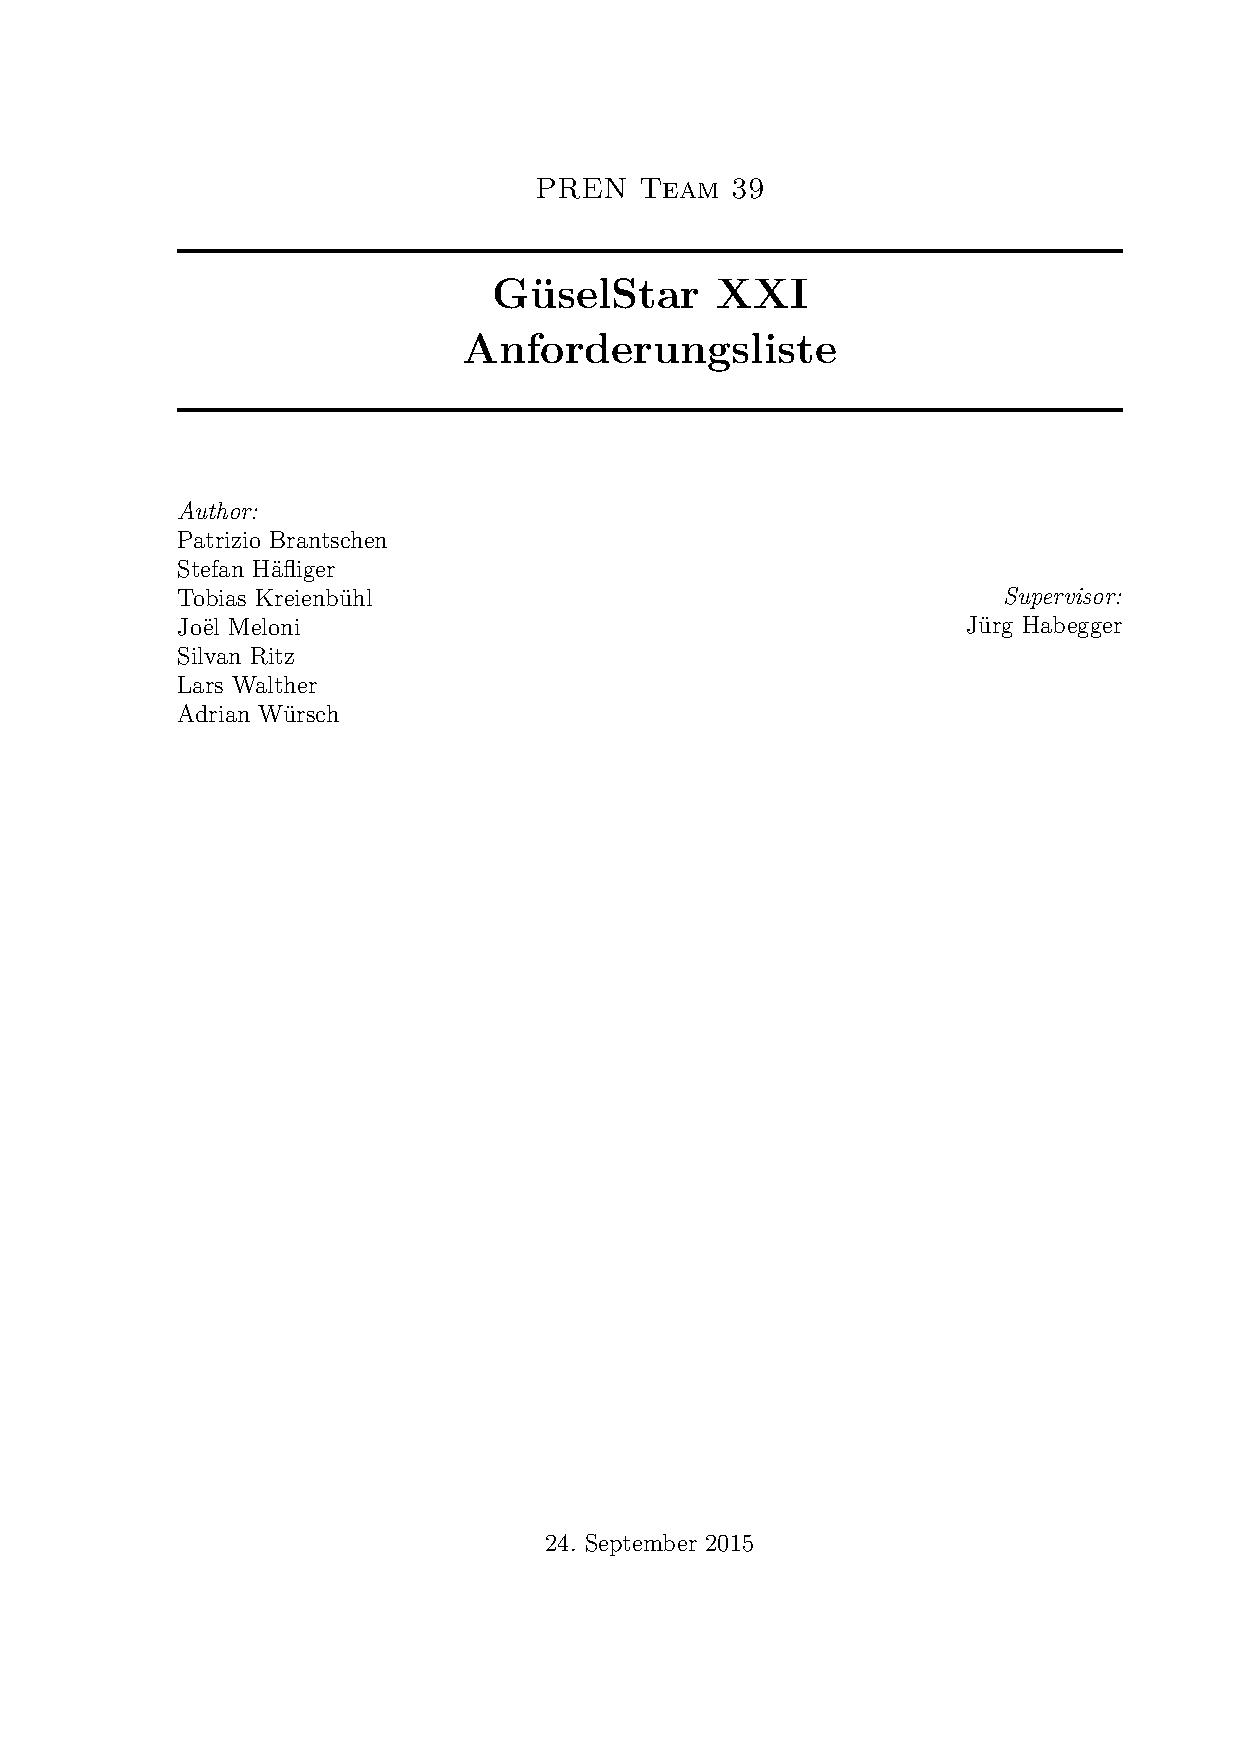
\includepdf[pages={-}]{../Anforderungsliste/Anforderungsliste.pdf}
\includepdf[pages={-}]{../MorphologischerKasten/morphkasten.pdf}



